\chapterhead{3}{Existence of the Canonical Subgroup: Applications}

In this chapter we study the "canonical subgroup\index{canonical subgroup}" of an elliptic curve\index{elliptic curve} whose
Hasse invariant\index{Hasse invariant} is "not too near zero." For simplicity, we assume throughout
this chapter that the grounding $R_0$ is a complete discrete valuation ring of
residue characteristic p and generic characteristic zero. We normalize the
ordinal function by requiring that $\ord(p)=1$.

\secmark{3.1}{The existence theorem: statement}

\begin{kathm}{Theorem}{3.1.}
(Lubin) I. Let $r\in R_0$ have $\ord(r)<p/p+1$. There is one and only one way
to attach to every r-situation $(E/R,\alpha_n,Y)$ (R a p-adically complete
$R_0$-algebra, $p\nmid n$, $n\geq 1$ if $p\neq 2,3$, $n\geq 3$ if $p=2,3$,
$Y\cdot E_{p-1}=r$) a finite flat rank p subgroup scheme $H\subset E$, called
the \uline{canonical subgroup} of $E/R$, such that:
\begin{quote}
$H$ depends only on the isomorphism class of $(E/R,\alpha_n,Y)$, and only on
that of $(E/R,Y)$ if $p\neq 2,3$.

The formation of $H$ commutes with arbitrary change of base $R\to R'$ of
p-adically complete $R_0$-algebras.

If $p/r=0$ in $R$, $H$ is the kernel of Frobenius\index{Frobenius}: $E\to E^{(p)}$.

If $E/R$ is the Tate curve\index{Tate curve} $\mathrm{Tate}(q^n)$ over $R_0/p^N R_0((q))$, then
$H$ is the subgroup $\mu_p$ of $\mathrm{Tate}(q^n)$.
\end{quote}
II. Suppose $r\in R_0$ has $\ord(r)<1/p+1$. Then there is one and only one way
to attach to every r-situation $(E/R,\alpha_n,Y)$ (R a p-adically complete
$R_0$-algebra, $p\nmid n$, $n\geq 1$ if $p\neq 2,3$, $n\geq 3$ if $p=2,3$,
$Y E_{p-1}=r$) an $r^p$-situation $(E'/R,\alpha_n',Y')$, where
\[
\begin{cases}
E' = E/H \\
\alpha_n' = \pi(\alpha_n), \quad \pi\colon E\to E' \text{ denoting the projection} \\
Y'\cdot E_{p-1}(E'/R,\alpha_n') = r^p
\end{cases}
\]
such that
\begin{quote}
$Y'$ depends only on the isomorphism class of $(E/R,\alpha_n,Y)$, and only on
that of $(E/R,Y)$ if $p\neq 2,3$.

The formation of $Y'$ commutes with arbitrary change of base $R\to R'$ of
p-adically complete $R_0$-algebras.

If $p/r=0$ in $R$, $Y'$ is the inverse image $Y^{(p)}$ of $Y$ on $E^{(p)}=E'$.
\end{quote}
\end{kathm}

Before giving the proof, we give some applications.

\secmark{3.2}{First principal corollary}

\begin{kathm}{Theorem}{3.2.}
Suppose $n\geq 3$, $p\nmid n$. Let $f$ be a modular form\index{modular form} of level n and weight
k on $\Gamma_0(p)$, defined over $R_0$, and which is holomorphic at the
unramified cusps of $\widetilde{M}_{n,p}$. There exists a (necessarily unique)
element $\widetilde{f}\in S(R_0,1,n,k)$ whose q-expansions at each cusp of
$\Mbar_n$ is that of $\widetilde{f}$ at the overlying unramified cusp of
$\widetilde{M}_{n,p}$. Furthermore, if $r\in R_0$ has $\ord(r)<p/p+1$, then in
fact $\widetilde{f}\in S(R_0,r,n,k)$.
\end{kathm}

\begin{kaproof}
Simply define $\widetilde{f}(E/R,\omega,\alpha_n,Y) = f(E/R,\omega,\alpha_n,H)$.
\end{kaproof}

\secmark{3.3}{Second principal corollary}

\begin{kathm}{Theorem}{3.3.}
Suppose $n\geq 3$, $p\nmid n$, and that either $k\geq 2$ or $k=1$ and
$n\leq 11$, or that $k=0$, $p\neq 2$, or that $k=0$, $p=2$ and $n\leq 11$. Let
$r\in R_0$ have $\ord(r)<1/p+1$. For any $f\in S(R_0,r^p,n,k)$, there is a
unique element $\varphi(f)\in S(R_0,1,n,k)$ whose q-expansions are given by
\[
\varphi(f)(\mathrm{Tate}(q^n),\omega_{can},\alpha_n) =
f(\mathrm{Tate}(q^{np}),\omega_{can},\pi(\alpha_n))
\]
[where $\pi\colon \mathrm{Tate}(q^n)\to\mathrm{Tate}(q^{np})$ is the map
"dividing by $\mu_p$", and $\pi(\alpha_n)$ is the induced level n-structure].
Furthermore, $\varphi(f)\cdot(E_{p-1})^k\in S(R_0,r,n,pk)$.
\end{kathm}

\begin{kaproof}
Define $\varphi(f)(E/R,\omega,\alpha_n,Y) = f(E'/R,\pi^*(\omega),\alpha_n',Y')$,
[$E'=E/H$, $\pi\colon E\to E'$ is the projection]. This makes sense if
$Y\cdot E_{p-1}=1$, for then $\pi$ is \'etale and so $\pi^*(\omega)$ is a
nowhere vanishing differential on $E'=E/H$. To see that
$E_{p-1}^k\cdot\varphi(f)$ actually lies in $S(R_0,r,n,kp)$, notice that its
value on $(E/R,\omega,\alpha_n,Y)$, $Y\cdot E_{p-1}=r^p$, is given formally by
$(E_{p-1}(E/R,\omega,\alpha_n))^k\cdot f(E'/R,\pi^*(\omega),\alpha_n',Y')$. [In
fact this expression has no meaning, because $\pi^*(\omega)$ may well
\uline{fail} to be nowhere-vanishing on $E'$.] However, if we write
$\pi^*(\omega)=\lambda\cdot\omega'$ with $\lambda\in R$ and $\omega'$
nowhere-vanishing on $E'$, then
\[
((E_{p-1})^k\cdot\varphi(f))(E/R,\omega,\alpha_n,Y) =
\left(\frac{E_{p-1}(E/R,\omega,\alpha_n)}{\lambda}\right)^k\cdot
f(E'/R,\omega',\alpha_n',Y').
\]
But a simple tangent calculation (cf. \eqref{ka:3.6.5}) shows that $\lambda$ and
$E_{p-1}$ are essentially equal; they differ multiplicatively by a unit of $R$.
By "reduction to the universal case", in which $R$ is flat over $\Z_p$, we can
make sense of the ratio $E_{p-1}/\lambda$, and interpret it as a unit in any
$R$; this permits us to define
$(E_{p-1})^k\cdot\varphi(f)(E/R,\omega,\alpha_n,Y) =
\left(\frac{E_{p-1}(E/R,\omega,\alpha_n)}{\lambda}\right)^k
f(E',\omega',\alpha_n',Y')$.
\end{kaproof}

\sechead{3.4}{Construction of the canonical subgroup in case $r=1$}

Let us first note that for $r=1$ the theorem is very simple. Given
$(E/R,\alpha_n)$ with $E_{p-1}(E/R,\alpha_n)$ invertible, the curve
$E\tens R/pR$ over $R/pR$ has invertible Hasse invariant\index{Hasse invariant}, hence
$\Ker(F\colon E\tens R/pR\to(E\tens R/pR)^{(p)})$ is a finite flat
subgroup-scheme of $E\tens R/pR$ of rank p whose Cartier dual, the kernel of
Verschiebung, is \uline{\'etale}. Since R is p-adically complete, Hensel's
lemma allows us to uniquely lift Ker F to the desired subgroup-scheme H of E/R
(by taking for H the Cartier dual of the unique lifting of its etale dual).
Since the Tate curve\index{Tate curve} $\mathrm{Tate}(q^n)$ over $\F_p((q))$ has
$\ker F = \mu_p$, the above argument shows that the canonical subgroup\index{canonical subgroup} of
$\mathrm{Tate}(q^n)$ over $R_0/p^N R_0((q))$ is $\mu_p$. This concludes the
proof of part I of the Theorem. For part II, still only in the case $r=1$, we
simply note that $E'=E/H$ reduces mod p to
$(E\tens R/pR)/\Ker F \simeq (E\tens R/pR)^{(p)}$, which certainly has
invertible Hasse invariant if $E\tens R/pR$ does - indeed
$E_{p-1}((E\tens R/pR)^{(p)},\omega^{(p)},\alpha_n^{(p)}) =
(E_{p-1}(E\tens R/pR,\omega,\alpha_n))^p$. Hence $E_{p-1}(E',\alpha_n')$ is
invertible in $R$. This concludes the proof of \eqref{ka:3.1} in the case $r=1$.

\secmark{3.5}{Hint for general $r$}

\kaitemb{3.5.0} The "general case" is unfortunately more difficult, and involves
a somewhat detailed study of the formal group\index{formal group} of an elliptic curve\index{elliptic curve}. Our method
of constructing the canonical subgroup will be to first construct a finite flat
subscheme of the formal group, then to show that it is in fact a subgroup which
has the desired properties. We begin with some lemmas on the formal group.

\sechead{3.6}{Lemmas on the formal group}

\begin{kathm}{Lemma}{3.6.1.}
Let R be an $\F_p$-algebra, E/R an elliptic curve\index{elliptic curve}, and $\omega$ a nowhere
vanishing differential. Let X be a parameter for the formal group\index{formal group} of E/R
(i.e., the completion of E along the identity section), which is \uline{dual}
to $\omega$ in the sense that the expansion of $\omega$ along the formal group
is
\[
\omega = (1 + \sum_{n\geq 1} a_n X^n)dX.
\]
Let $A(E,\omega)$ denote the Hasse invariant\index{Hasse invariant}. Then we have the identities
\[
a_{p^n-1} = (A(E,\omega))^{\frac{p^n-1}{p-1}} \quad\text{for}\quad n=1,2,\dots.
\]
\end{kathm}

\begin{kaproof}
Let $\cC\colon \Omega^1_{E/R}\to(\Omega^1_{E/R})^{(p)}$ denote the Cartier
operator, "dual" to the endomorphism $D\to D^p$ of $T_{E/R}$. We have
$\cC(\omega) = A(E,\omega)\cdot\omega^{(p)}$, but we may calculate $\cC$
"locally":
\[
\cC(a_n X^n dX) = \begin{cases} 0, & p\nmid n+1 \\ a_n(X^{\frac{n+1}{p}-1}dX)^{(p)} & \text{if } p\mid n+1 \end{cases}
\]
Hence $\cC(\omega) = \sum_{m\geq 0} a_{p(m+1)-1}(X^m dX)^{(p)}$, and
$\cC(\omega) = A(E,\omega)\cdot\omega^{\otimes p} =
\sum A(E,\omega)(a_m)^p(X^m dX)^{(p)}$, whence
$a_{p(m+1)-1} = A(E,\omega)\cdot(a_m)^p$. As $a_0=1$, the result follows easily.
\end{kaproof}

\begin{kathm}{Lemma}{3.6.2.}
Let R be any $\Z_p$-algebra, and let G be a one-parameter formal group over R.
Then
\begin{quote}
(1) $\End_R(G)\supset \Z_p$ and $\Z_p$ lies in the center of $\End_R(G)$.

(2) Given any parameter $X_0$, there exists a (non-unique!) parameter
$X = X_0 +$ higher terms such that for any p-1'st root of unity $\zeta\in\Z_p$,
we have $[\zeta](X) = \zeta X$.
\end{quote}
\end{kathm}

\begin{kaproof}
Thanks to Lazard, we're reduced to the universal situation, which has R flat
over $\Z_p$. So we may use log, exp, and continuity to get (1). As for (2), it
is proven directly in (\cite{lubin64}, lemma 4.12), or we can remark that \uline{any}
choice of a "p-typical coordinate" X (cf.\cite{cartier67}, \cite{cartier72}) which is congruent to $X_0$
mod degree two terms will do the job.
\end{kaproof}

\begin{kathm}{Lemma}{3.6.3.}
Let R be an $\F_p$-algebra, G a one-parameter formal group over R. In terms of
any parameter X, $[p](X)$ is a function of $X^p$: i.e.
\begin{kadispb}{3.6.3.0}
[p](X) = V(X^p) = \sum_{n\geq 1} v_n X^{np}.
\end{kadispb}
\end{kathm}

\begin{kaproof}
In $\End_R(G)$, $p = V\circ F$, $F\colon G\to G^{(p)}$, $V\colon G^{(p)}\to G$.
\end{kaproof}

\begin{kathm}{Lemma}{3.6.4.}
Let R be a $\Z_p$-algebra, G a one-parameter formal group over R, X a parameter
on G such that $[\zeta](X) = \zeta X$ for any p-1'st root of unity
$\zeta\in\Z_p$. Then $[p](X) = X\cdot(\text{a series in } X^{p-1})$.
\end{kathm}

\begin{kaproof}
$[p]([\zeta](X)) = [\zeta]([p](X))$ because $p\cdot\zeta = \zeta\cdot p$ in
$\Z_p$. Thus $[p](\zeta X) = \zeta\cdot([p](X))$, so writing
$[p](X) = \sum e_n X^n$, we have $e_n\zeta^n = e_n\zeta$, hence
$(\zeta-\zeta^n)e_n = 0$. But for $n\neq 1$ (p-1), $\zeta-\zeta^n$ is
\uline{invertible} in $\Z_p$, hence $e_n = 0$.
\end{kaproof}

\begin{kathm}{Lemma}{3.6.5.}
Let R be a $\Z_p$-algebra, G a one-parameter formal group over R, X a
parameter, $\omega = (1 + \sum_{n\geq 1} a_n X^n)dX$ the dual invariant
differential. Then we have
\begin{kadispb}{3.6.5.0}
[p](X) \equiv a_{p-1}\cdot X^p + \text{higher terms } \bmod(p).
\end{kadispb}
\end{kathm}

\begin{kaproof}\relax
[In the application to elliptic curves, we have $a_{p-1} = A(E,\omega)$, and
$[p](X) = V(X^p) = \text{tangent}(V)\cdot X^p + \text{higher terms}$, so the
assertion is that $A(E,\omega) = \text{tangent}(V) = \text{action of } F$ on
$H^1(E,\cO)$, which is true!]

By Lazard, we are reduced to the universal case, in which R is flat over
$\Z_p$. Over $R[1/p]$, we have $\omega = d\varphi(X)$, $\varphi(X)\in
R[1/p][[X]]$, $\varphi(X) = X + \sum_{n=2}^{p-2} a_n\frac{X^{n+1}}{n+1} +
a_{p-1}\frac{X^p}{p} + \text{higher terms}$. Let $\psi(X)$ be the inverse
series to $\varphi$: $\psi(X) = X + \cdots, \psi(\varphi(X)) = X$. Then
$[p](X) = \psi(p\cdot\varphi(X))$.

Because $\varphi(X)$ mod degree p lies in $X + X^2R[[X]]$, for each $n\geq 2$,
$\varphi(X)^n$ mod degree $p+1$ lies in $X^n + X^{n+1}R[[X]]$. If we write
$\psi(X) = X + \sum_{i\geq 2} b_i X^i$, we see from this and the requirement
$\psi(\varphi(X)) = X$ that $b_2,\dots,b_{p-1}\in R$, while
$b_p = -\frac{a_{p-1}}{p}$ modulo R. Now the term of degree p in
$[p](X) = \psi(p\varphi(X))$ is given by
\[
\sum_{i=1}^{p} b_i p^i\cdot(\text{coef of } X^p \text{ in } (\varphi(X))^i) =
a_{p-1} + \sum_{i=2}^{p-1} b_i p^i(\text{coef of } X^p \text{ in }
\varphi(X)^i) + b_p\cdot p^p,
\]
and as $p b_p\in R$, we see that \uline{all} the terms save $a_{p-1}$ lie in
$pR$.
\end{kaproof}

We may summarize our findings in a proposition.

\begin{kathm}{Proposition}{3.6.6.}
Let R be a $\Z_p$-algebra, G a one-parameter formal group over R, X a
coordinate on G which satisfies $[\zeta](X) = \zeta X$ for every p-1'st root of
unity $\zeta\in\Z_p$, and $\omega$ the "dual" differential. Then
\begin{kadispb}{3.6.6.0}
[p](X) = pX + aX^p + \sum_{m\geq 2} c_m\cdot X^{m(p-1)+1}
\end{kadispb}
where $a,c_2,c_3,\dots,\in R$, and $c_m\in pR$ \uline{unless}
$m(p-1)+1\equiv 0\ (p)$, i.e., $c_m\in pR$ unless $m\equiv 1\ (p)$. Further,
if G is the formal group of an elliptic curve E/R, then
$a\equiv A(E,\omega)\bmod pR$.
\end{kathm}

\begin{kaproof}
By \eqref{ka:3.6.4}, $[p](X) = X\cdot(\text{a series in } X^{p-1})$, but modulo $pR$,
$[p](X)$ is also a series in $X^p$, by \eqref{ka:3.6.3}. The congruence for $a$ is by
\eqref{ka:3.6.1}.
\end{kaproof}

\sechead{3.7}{Construction of the canonical subgroup as a subscheme of the formal group}

Suppose we are given $(E/R,\alpha_n,Y)$ with R a p-adically complete
$R_0$-algebra, $n\geq 1$ if $p\neq 2,3$, $n\geq 3$ for $p=2,3$,
$Y\cdot E_{p-1}=r$, $\ord(r)<p/p+1$. Because it suffices to treat the case when
p is nilpotent in R, we may, by ordinary localization on R, suppose that the
formal group\index{formal group} of E/R is given by a one-parameter formal group law over R, with
formal paramter X; we denote by $\omega$ the "dual" differential. By reduction
to the universal case, we may \uline{now} reduce to the case when R is a
\uline{flat} $\Z_p$-algebra. By \eqref{ka:3.6.2}, we may suppose that
$[\zeta](X) = \zeta X$ for all p-1'st roots of unity $\zeta\in\Z_p$. By
\eqref{ka:3.6.6}, the endomorphism $[p]$ on the formal group looks like
\begin{kadisp}{3.7.0}
[p](X) = pX + aX^p + \sum_{m\geq 2} c_m X^{m(p-1)+1}
\end{kadisp}
\[
\text{with}\quad \begin{cases}
a \equiv E_{p-1}(E/R,\omega,\alpha_n) \bmod pR \\
c_m \equiv 0 \bmod pR \text{ unless } m\equiv 1\ (p).
\end{cases}
\]

We first give a heuristic for the method to be used.

Naively speaking, the kernel of $[p]$ is an $\F_p$-vector space, and the
canonical subgroup\index{canonical subgroup} is just a nice choice of a \uline{line} in this
$\F_p$-space, i.e., it is an \uline{orbit} of $\F_p^\times$ in this vector
space. But the action of $\F_p^\times$ on $\Ker([p])$ is induced by the action
of $\mu_{p-1}\subset\Z_p$ on the formal group. Thus we must write down the
\uline{equation} for the \uline{orbits} of the action of $\mu_{p-1}$ on
$\Ker([p])$, and somehow solve this equation in a "canonical" way. Because
$\zeta\in\mu_{p-1}$ acts on X by $[\zeta](X) = \zeta X$, it is natural to take
$T\xlongequal{\mathrm{dfn}} X^{p-1}$ as a parameter for the space of orbits of
the action of $\F_p^*$ on $\Ker([p])$. The formal identity (obtained from
\eqref{ka:3.6.6.0} by substituting $T = X^{p-1}$)
\begin{kadisp}{3.7.1}
[p](X) = X\cdot(p + aT + \sum_{m\geq 2} c_m T^m)
\end{kadisp}
suggests that in fact the equation for the orbits is
\begin{kadisp}{3.7.2}
g(T) \xlongequal{\mathrm{dfn}} p + aT + \sum_{m\geq 2} c_m T^m = 0,
\end{kadisp}
and that the canonical subgroup is nothing more than a canonical zero of
$g(T)$.

We now implement the above heuristically-motivated procedure. Let
$r_1\in R_0$ be the element $-p/r$; we have
$\ord(r_1) = 1 - \ord(r) > 1/p+1$, (because $\ord(r)<p/p+1$ by hypothesis). Let
$Y = Y(E/R,\omega,\alpha_n)\in R$; we have $Y\cdot E_{p-1}(E/R,\omega,\alpha_n)
= r$. Because $a\equiv E_{p-1}(E/R,\omega,\alpha_n)$ modulo $pR$, we may write
$E_{p-1}(E/R,\omega,\alpha_n) = a+pb$, $b\in R$. Thus $Y\cdot(a+pb) = r$, and an
immediate calculation shows that if we put
\begin{kadisp}{3.7.4}
t_0 = \frac{r_1 Y}{1 + r_1 bY}
\end{kadisp}
(which makes sense, because $r_1$ is topologically nilpotent in R), then
$p + at_0 = 0$.

Let's define $g_1(T) = g(t_0 T)$;
\begin{kadisp}{3.7.5}
g_1(T) &= p + at_0 T + \sum_{m\geq 2} c_m(t_0)^m T^m \\
&= p - pT + \sum_{r\geq 2} c_r(t_0)^m T^m.
\end{kadisp}

Let $r_2 = (r_1)^{p+1}/p$, an element of $R_0$ having $\ord(r_2)>0$. Let
$r_3\in R_0$ be any generator of the ideal $(r_2,(r_1)^2)$ of $R_0$.

\begin{kathm}{Lemma}{3.7.6.}
We may write $g_1(T) = p\cdot g_2(T)$, with
\begin{kadisp}{3.7.6.1}
g_2(T) = 1 - T + \sum_{m\geq 2} d_m T^m,
\end{kadisp}
with $d_m\in r_3 R$, and $d_m\to 0$ as $m\to\infty$.
\end{kathm}

\begin{kaproof}
We have $d_m = c_m(t_0)^m/p$. Because $c_m/p$ lies in R if $m\not\equiv 1 \bmod
p$, and because $(t_0)^{p+1}/p$ lies in $r_2 R$, we have $d_m\in r_3 R$ for all
$m\geq 2$, and $d_m\to 0$ as $m\to\infty$. We next apply Newton's lemma to R,
$I = r_3 R$ and $h = g_2$.
\end{kaproof}

\begin{kathm}{Lemma}{3.7.7.}
(Newton) Let R be a ring complete and separated with respect to powers of an
ideal $I\subset R$. Let $h(T) = 1 - T + \sum_{m=2}^{\infty} d_m T^m$, with
$d_m\in I$, and $d_m\to 0$ as $m\to\infty$. By "substitution", h gives rise to
a continuous function $h\colon R\to R$. There exists a unique element
$t_\infty\in I$ such that $h(1 - t_\infty) = 0$.
\end{kathm}

\begin{kaproof}
Making the substitution $T = 1-S$, we introduce
$h_1(S) = h(1-S) = e_0 + (1+e_1)S + \sum_{m\geq 2} e_m S^m$, with coefficients
$e_i\in I$. For $s\in I$, $h_1(s) = h(1-s)$, so our problem is to show that
$h_1$ has a unique zero $s_\infty$ in I. For any $s\in I$, $h_1'(s)\in 1+I$,
hence is invertible in R, while $h_1(s)\in I$. The Newton process of successive
approximations: $s_0 = 0,\dots,s_{n+1} = s_n - h_1(s_n)/h_1'(s_n)$ is easily
seen to converge to a zero of $h_1$. If $s$ and $s+\Delta$ are \uline{two}
zeros of $h_1$ in I, we have
$0 = h_1(s+\Delta) = h_1(s) + h_1'(s)\cdot\Delta + (\Delta^2) = h_1'(s)\cdot
\Delta + (\Delta^2)$, hence as $h_1'(s)$ is invertible, we have
$\Delta\in(\Delta^2)$. Because $\Delta\in I$ and R is I-adically separated,
this implies $\Delta = 0$.
\end{kaproof}

Tracing back our steps, we have constructed a zero $t_{can} = t_0(1 - t_\infty)$
of $g(T)$. Because $t_{can}$ lies in $r_1 R$, we may expand g in powers of
$T-t_\infty$, and conclude that $g(T)$ is \uline{divisible} by $T-t_{can}$ in
$R[[T]]$. We \uline{define} the \uline{canonical subscheme} to be the finite
flat rank p subscheme of $\Ker([p])$ defined by the equation $X^p - t_{can}X$.
(It may be verified that this subscheme is \uline{independent} of the choice of
coordinate X on the formal group satisfying $[\zeta](X) = \zeta X$ for all
p-1'st roots of unity $\zeta\in\Z_p$.)

\sechead{3.8}{The canonical subscheme is a subgroup}

Let's begin by remarking that if E/R modulo p has \uline{invertible} Hasse
invariant, then $[p](X) = pX + (\text{unit})X^p + \cdots$. By the formal version
of the Weierstrass Preparation Theorem, we see that in $R[[X]]$, we have
$[p](X) = (X^p - t_{can}X)\cdot(\text{a unit in } R[[X]])$. Thus when Hasse is
invertible mod p, the canonical subscheme is \uline{all} of $\Ker([p])$ in the
formal group\index{formal group}, hence in particular it's a subgroup-scheme of the formal group.

In the general case, the condition that the subscheme of equation
$X^p - t_{can}X$ be a subgroup-scheme of the formal group is that, noting by
$G(X,Y)$ the group law, we have
\begin{kadisp}{3.8.1}
G(X,Y)^p - t_{can}G(X,Y) = 0 \quad\text{in}\quad R[[X,Y]]/(X^p - t_{can}X, Y^p - t_{can}Y).
\end{kadisp}
Because $t_{can}$ lies in $r_1 R$, it is topologically nilpotent in R, hence
the R-algebra $\cA = R[[X,Y]]/(X^p - t_{can}X, Y^p - t_{can}Y)$ is finite and
free of rank $p^2$ with basis $X^i Y^j$, $0\leq i$, $j\leq p-1$. The condition
that $G(X,Y)^p - t_\infty G(X,Y)$ vanish in $\cA$ is simply that the $p^2$
"coefficients" $g_{i,j}\in R$ defined by the equation
\begin{kadisp}{3.8.2}
G(X,Y)^p - t_\infty G(X,Y) = \sum_{0\leq i,j\leq p-1} g_{i,j}X^i Y^j \quad\text{in } \cA
\end{kadisp}
all \uline{vanish} in R. Thus it suffices to find a p-adically complete
$R_0$-algebra $R'\supset R$ such that, \uline{over $R'$}, the canonical
subscheme is a subgroup (for then the $g_{i,j}$ vanish in $R'$, hence vanish in
R). But in the universal situation, $R = M(R_0,r,n,0)\subset R' =
M(R_0,1,n,0)$, and over $R'$, $E_{p-1}$ is invertible, hence Hasse mod p is
invertible, and so as noted above the canonical subscheme \uline{is} a subgroup
over $R'$. This concludes the proof of part I of the main theorem \eqref{ka:3.1}.

\secmark{3.9}{Conclusion of the proof of 3.1}

\kaitem{3.9} We now turn to proving part II of 3.1, by constructing $Y'$. As
before we may suppose R flat over $\Z_p$. Let $r\in R_0$ have $\ord(r)<1/p+1$.
Then $r_1 = p/r$ has $\ord(r_1)>p/p+1$, and hence $r_1$ is \uline{divisible} by
$r^p$, and $r_4 = r_1/r^p$ has $\ord(r_4)>0$. Since $t_{can}\in r_1 R$, modulo
$r_1 R$ the canonical subgroup\index{canonical subgroup} is just the kernel of $F\colon E\to E^{(p)}$.
Hence $E'$ mod $r_1 R$ is $E^{(p)}$. Let $\omega'$ be any nowhere vanishing
one-form on $E'$ which reduces modulo $r_1 R$ to $\omega^{(p)}$ on $E^{(p)}$.
Hence we have the congruence
\begin{kadisp}{3.9.1}
E_{p-1}(E'/R,\omega',\alpha_n') \equiv (E_{p-1}(E/R,\omega,\alpha_n))^p \text{ modulo } r_1 R.
\end{kadisp}
Because $r_1 = r_4\cdot r^p$, we may write
\begin{kadisp}{3.9.2}
E_{p-1}(E'/R,\omega',\alpha_n') = (E_{p-1}(E/R,\omega,\alpha_n))^p + r^p r_4 j, \quad j\in R.
\end{kadisp}
Using the equation
\begin{kadisp}{3.9.3}
Y(E/R,\omega,\alpha_n)\cdot E_{p-1}(E/R,\omega,\alpha_n) = r
\end{kadisp}
one immediately checks that if we define
\begin{kadisp}{3.9.4}
Y'(E'/R,\omega',\alpha_n') = \frac{(Y(E/R,\omega,\alpha_n))^p}{1 + r_4 j\cdot(Y(E/R,\omega,\alpha_n))^p},
\end{kadisp}
then $Y'(E'/R,\omega',\alpha_n')\cdot E_{p-1}(E'/R,\omega',\alpha_n') = r^p$.
This concludes the proof of part II. \hspace*{\fill}$\square$

\sechead{3.10}{Finiteness properties of the Frobenius endomorphism of p-adic modular functions.}

Throughout the rest of this chapter, we denote by $R_0$ a complete discrete
valuation ring of mixed characteristic with \uline{perfect} residue field
$R_0/\mathfrak{m}$. The \uline{Frobenius\index{Frobenius} endomorphism} $\varphi$ of
$S(R_0,1,n,k)$ is defined by
$\varphi(f)(E,\omega,\alpha_n,Y=(E_{p-1})^{-1}) =
f(E/H,\pi^*(\omega),\pi(\alpha_n),Y'=1/E_{p-1})$, where H denotes the
canonical subgroup\index{canonical subgroup} of E, $\pi\colon E\to E/H$ denotes the projection. As we
have seen above, for $r\in R_0$ having $\ord(r)<1/p+1$, the composite
$(E_{p-1})^k\cdot\varphi$ "extends" to give a commutative diagram
\begin{equation}\tag*{3.10.0}\label{ka:3.10.0}
\begin{tikzcd}
S(R_0,1,n,k) \arrow[r,"\varphi"] \arrow[d,hook] & S(R_0,1,n,k) \arrow[r,"(E_{p-1})^k"] & S(R_0,1,n,pk) \arrow[d,hook] \\
S(R_0,r^p,n,k) \arrow[rr,dashed] & & S(R_0,r,n,pk)
\end{tikzcd}
\end{equation}
For $k=0$, we find simply that the endomorphism $\varphi$ maps
$S(R_0,r^p,n,0)$ to $S(R_0,r,n,0)$ for any $r\in R_0$ having
$\ord(r)<1/p+1$.

\begin{kathm}{Theorem}{3.10.1.}
Suppose $n\geq 3$ and $p\nmid n$, and $n\leq 11$ if $p=2$. Then
\begin{quote}
I. For $r\in R_0$ with $\ord(r)<1/p+1$, the Frobenius morphism
$\varphi\colon S(R_0,r^p,n,0)\to S(R_0,r,n,0)$ is a \uline{finite} morphism
(but \uline{not} in general flat).

II. If $r=1$, then $\varphi$ is a finite flat morphism of degree p.

III. For \uline{any} $r$ with $\ord(r)<1/p+1$, the homomorphism (K the
fraction field of $R_0$)
\[
\varphi\tens K\colon S(R_0,r^p,n,0)\tens K\to S(R_0,r,n,0)\tens K
\]
is finite and etale of rank p.
\end{quote}
\end{kathm}

\begin{kaproof}
(I). Because the ring $S(R_0,r,n,0)$ is complete and separated in the p-adic
topology, to prove finiteness of $\varphi$ it suffices to prove that the
induced homomorphism
\begin{kadispb}{3.10.2}
\varphi\tens R_0/\mathfrak{m}\colon S(R_0,r^p,n,0)\tens R_0/\mathfrak{m}\to S(R_0,r,n,0)\tens R_0/\mathfrak{m}
\end{kadispb}
is finite. Interpreting $S(R_0,r,n,0)$ as $H^0(\Mbar_n(R_0,r),\cO)$ (cf. \eqref{ka:2.9}),
and noting that $\Mbar_n(R_0,r)$ is \uline{flat} over $R_0$, we see (by
"universal coefficients") that the canonical homomorphism
$S(R_0,r,n,0)\tens R_0/\mathfrak{m}\to S(R_0/\mathfrak{m},r,n,0)$ is
\uline{injective}, with cokernel of finite dimension over $R_0/\mathfrak{m}$.
Thus $S(R_0/\mathfrak{m},r,n,0)$ is a finite module over
$S(R_0,r,n,0)\tens R_0/\mathfrak{m}$, and we have a commutative diagram of ring
homomorphisms
\begin{equation}\tag*{3.10.3}\label{ka:3.10.3}
\begin{tikzcd}
S(R_0/\mathfrak{m},r^p,n,0) \arrow[r,"\varphi"] & S(R_0/\mathfrak{m},r,n,0) \\
S(R_0,r^p,n,0)\tens R_0/\mathfrak{m} \arrow[r,"\varphi\tens R_0/\mathfrak{m}"] \arrow[u,hook] & S(R_0,r,n,0)\tens R_0/\mathfrak{m} \arrow[u,hook]
\end{tikzcd}
\end{equation}
in which the vertical arrows are \uline{finite}. Thus the finiteness of the
lower horizontal arrow (which is what we wish to prove) follows from the
finiteness of the upper horizontal arrow.

Notice that if $r=1$, both $S(R_0/\mathfrak{m},r,n,0)$ and
$S(R_0/\mathfrak{m},r^p,n,0)$ are $S(R_0/\mathfrak{m},1,n,0)$, while if
$0<\ord(r)$, both $S(R_0/\mathfrak{m},r,n,0)$ and $S(R_0/\mathfrak{m},r^p,n,0)$
are $S(R_0/\mathfrak{m},0,n,0)$. Because $\ord(r)<1/p+1$, both $p/r$ and
$p/r^p$ lie in $\mathfrak{m}$, and hence over $R_0/\mathfrak{m}$ the canonical
subgroup over $\Mbar_n(R_0/\mathfrak{m},r)$ and over
$\Mbar_n(R_0/\mathfrak{m},n,r^p)$ is just the \uline{kernel of Frobenius}. It
follows immediately that in either case (i.e., $r=1$ or $0<\ord(r)<1/p+1$),
the \uline{endomorphism} $\varphi$ of $S(R_0/\mathfrak{m},r,n,0)$ is precisely
the p'th power mapping (because
$\varphi(f)(E,\omega,\alpha_n,Y) = f(E^{(p)},\omega^{(p)},\alpha_n^{(p)},Y' ={}\allowbreak
Y(E,\omega,\alpha_n)^p) = (f(E,\omega,\alpha_n,Y))^p)$. But
$\Mbar_n(R_0/\mathfrak{m},r)$ is a scheme of finite type over
$R_0/\mathfrak{m}$, hence $S(R_0/\mathfrak{m},r,n,0)$ is a finitely generated
$R_0/\mathfrak{m}$-algebra, hence finite over itself by the p'th power
endomorphism, which proves (I).

For (II), we remark that when $r=1$, the scheme
$\Mbar_n(R_0/\mathfrak{m},1)$ is simply the open set of
$\Mbar_n\tens R_0/\mathfrak{m}$ where $E_{p-1}$ is invertible, hence is a
\uline{smooth affine curve} over $R_0/\mathfrak{m}$. Hence the p'th power
endomorphism of its coordinate ring $S(R_0/\mathfrak{m},1,n,0)$ makes that ring
finite and flat over itself of rank p. Because $S(R_0,1,n,0)$ is p-adically
complete and flat over $R_0$, it follows that $\varphi$ makes $S(R_0,1,n,0)$
into a finite flat module over itself of degree p.

The proof of (III) is more difficult, and requires Tate's theory of rigid
analytic spaces. The ring $S(R_0,r,n,0)$ is the p-adic completion of
$H^0(\Mbar_n\tens R_0,\Sym(\w^{\otimes p-1}))/(E_{p-1}-r)$, and this last
algebra is \uline{finitely generated} over $R_0$ (because $\w$ has positive
degree, hence is \uline{ample}). Thus noting by K the fraction field of $R_0$,
we see that $S(R_0,r,n,0)\tens K$ is a \uline{rigid algebra} in the sense of
Tate, and contains as \uline{dense} subalgebra the K-algebra
\[
\begin{gathered}
H^0(\Mbar_n\tens K,\Sym(\w^{\otimes p-1}))/(E_{p-1}-r) \simeq
H^0(\Mbar_n\tens K,\Sym(\w^{\otimes p-1}))/(E_{p-1}-1)\\
\simeq
H^0(\Mbar_n\tens K,\Sym(\w^{\otimes p-1}))/(E_{p-1}-1),
\end{gathered}
\]
which is precisely the \uline{coordinate ring} $D_n\tens K$ of the open subset
of $\Mbar_n\tens K$ where $E_{p-1}$ is \uline{invertible}. Thanks to Tate, the
\uline{ideals} of $S(R_0,r,n,0)\tens K$ are all \uline{closed}, hence are the
closures of their intersections with $D_n\tens K$. But as $D_n\tens K$ is the
coordinate ring of a smooth affine curve over K, its prime ideals are either
\uline{minimal} (corresponding to irreducible components) or \uline{maximal}
(corresponding to conjugacy classes of points with values in finite extensions
of K). Indeed, the closed points of $S(R_0,r,n,0)\tens K$ are conjugacy
classes of homomorphisms $\pi\colon S(R_0,r,n,0)\to K'$, $K'$ a finite
extension of K, or equivalently they are homomorphisms
$\pi\colon D_n\tens K\to K'$ which satisfy the continuity conditions
$|\pi(D_n)|\leq 1$, $1\geq|\pi(E_{p-1})|\geq|r|$ (i.e., that the images of
$E_{p-1}$ and of $Y = r/E_{p-1}$ be "power bounded"). Further, the completions
of the local rings at corresponding closed points are isomorphic, hence are
regular local rings of dimension one, hence $S(R_0,r,n,0)\tens K$ is a
\uline{regular ring of dimension one}. Thus the map
\begin{kadispb}{3.10.4}
S(R_0,r^p,n,0)\tens K \xrightarrow{\varphi\tens K} S(R_0,r,n,0)\tens K
\end{kadispb}
is a \uline{finite} morphism between regular rings of the same dimension, hence
(cf. EGA IV,17.3.5.2) is \uline{flat}. To see that it has rank p, it suffices
to note that by (II), it has rank p over the dense open set where
$|E_{p-1}|=1$. It remains only to see that \eqref{ka:3.10.4} is \uline{\'etale}. For
this, it suffices to show that the \uline{fibre} over each point with values in
$\Omega$, the completion of the algebraic closure of K, consists of p distinct
points. Over a point at \uline{infinity}, corresponding to
$\mathrm{Tate}(q^n)$ over $K((q))$, the fibre consists of the p curves
$\mathrm{Tate}(\zeta_p q^{n/p})$ over $K((q))$, each of which gives rise to
$\mathrm{Tate}(q^n)$ upon division by its canonical subgroup $\mu_p$. A
\uline{finite} point is an elliptic curve\index{elliptic curve} $E/\Omega$ [with level n structure
$\alpha_n$] having good reduction, such that for any differential $\omega$
which extends to a nowhere vanishing differential over the valuation ring of
$\Omega$, we have $1\geq|E_{p-1}(E/K,\omega)|\geq|r|^p$. The curve E has p+1
subgroups of order p, say $H_0,H_1,\dots,H_p$, of which $H_0$ is the
\uline{canonical} subgroup.

Let $E^{(1)} = E/H_1$. The points lying over E are \uline{among} the p+1
curves $E^{(i)}$, ($E^{(i)}$ carrying the induced level n structure); indeed,
$E^{(i)}$ lies over if and only if $E^{(i)}$ \uline{is} a point of
$S(R_0,r,n,0)\tens\Omega$ whose canonical subgroup is $E/H_1$.

Consider first the case in which $|E_{p-1}(E/K,\omega)|=1$, i.e., a formal
group of height one. Then $H_0$ \uline{is} the kernel of p in the formal
group, while the $H_i$, $i\geq 1$, meet the formal group\index{formal group} only in $\{0\}$. The
quotient $E^{(0)} = E/H_0$ again has a formal group of "height one" hence its
canonical subgroup is the kernel of p in \uline{its} formal group, while the
image of $E$ in $E^{(0)}$ meets the formal group only in $\{0\}$. Thus
$E^{(0)}$ does \uline{not} lie over E. For $i\geq 1$, the quotient $E^{(i)}$
also has a formal group of height one, but now the image of $H_0$ in
$E^{(i)} = E/H_i$ \uline{is} the kernel of p in the formal group, i.e., it is
the canonical subgroup, and hence the $E^{(i)}$, $i=1,\dots,p$, do lie over.

It remains to treat the case of "supersingular reduction", which we do by
Lubin's original method, and show (part 5 of theorem 3.10.7) that again only
$E^{(1)},\dots,E^{(p)}$ lie over.
\end{kaproof}

\kaitem{3.10.5} Let $\Omega$ be an algebraically closed complete (under a rank
one valuation) field of characteristic zero and residue characteristic p. Let
$R\subset K$ be the valuation ring, and let $E/R$ be an elliptic curve over R,
and X a parameter for the formal group of E/R, normalized by the condition
$[\zeta](X) = \zeta X$ for every p-1'st root of unity in $\Z_p$. Suppose that
the Hasse invariant\index{Hasse invariant} of the special fibre vanishes. Then in the formal group, we
have
\begin{kadisp}{3.10.6}
[p](X) = pX + aX^p + \sum_{m=2}^{p} c_m X^{m(p-1)+1} + c_{p+1}X^{p^2} + \sum_{m\geq p+2} c_m X^{m(p-1)+1}
\end{kadisp}
with $\ord(a)>0$, $\ord(c_m)\geq 1$ for $m\not\equiv 1 \bmod p$, and
$\ord(c_{p+1}) = 0$, (this last because we suppose height two for the special
fibre). [If $\ord(a)<1$, we have $\ord(a) = \ord E_{p-1}(E/R,\omega)$ for any
nowhere vanishing differential $\omega$ on E/R, by \eqref{ka:2.1}.]

\begin{kathm}{Theorem}{3.10.7.}
(Lubin)
\begin{quote}
1. If $\ord(a)<p/p+1$, the canonical subgroup $H_0$ consists of $\{0\}$ and
the p-1 solutions X of \eqref{ka:3.10.6} whose ordinal is $\frac{1-\ord(a)}{p-1}$. The
$p^2-p$ other solutions of \eqref{ka:3.10.6} all have ordinal
$\frac{\ord(a)}{p^2-p}$ (which is $<\frac{1-\ord(a)}{p-1}$). If
$\ord(a)\geq p/p+1$, then \uline{all} non-zero solutions of \eqref{ka:3.10.6} have
ordinal $1/p^2-1$.

2. If $\ord(a)<1/p+1$, then the quotient $E' = E/H_0$ has as normalized
coordinate for its formal group $X' = \prod_{x\in H_0} G(X,x)$, where $G(X,Y)$
denotes the formal group law on E. The expression of $[p]$ on $E/H_0$ is
\[
[p](X') = pX' + a'(X')^p + \cdots
\]
with $\ord(a') = p \ord(a)$.

3. If $1/p+1<\ord(a)<p/p+1$, then $\ord(a') = 1 - \ord a$, and the
\uline{canonical subgroup} of $E/H_0$ is $E/H_0$, and $(E/H_0)/H_0(E/H_0)$ is
just E, (but a level n structure $\alpha_n$ becomes $p^{-1}\cdot\alpha_n$ after
two divisions by the canonical subgroup - (compare Dwork \cite{dwork69}, 8.11)).

4. If $\ord(a)\geq p/p+1$, there exist p+1 curves $E^{(i)}$, each having
$\ord(a^{(i)}) = 1/p+1$, such that $E = E^{(i)}/H_0(E^{(i)})$, where
$H_0(E^{(i)})$ denotes the \uline{canonical subgroup} of $E^{(i)}$. These
curves are $E^{(i)} = E/H_i$, $i=0,1,\dots,p$.

5. If $0<\ord(a)<p/p+1$, there exist precisely p curves $E^{(i)}$ having
$\ord(a_i)<1/p+1$ such that $E = E^{(i)}/H_0(E^{(i)})$, namely the curves
$E^{(i)} = E/H_i$, $i=1,\dots,p$ (cf.\eqref{ka:3.10.4}ff), and
$\ord(a_i) = \frac{1}{p}\ord(a)$.
\end{quote}
\end{kathm}

\begin{kaproof}
1. follows from looking at the Newton polygon\index{Newton polygon} of $[p](X)$, which is
\begin{center}
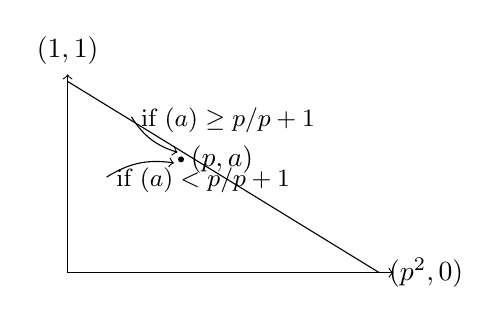
\begin{tikzpicture}[scale=0.9]
\draw[->] (0,0) -- (4.6,0) node[right]{};
\draw[->] (0,0) -- (0,2.8);
\node[above] at (0,2.8) {$(1,1)$};
\draw (0,2.7) -- (4.4,0);
\node[right] at (4.4,0) {$(p^2,0)$};
\fill (1.6,1.6) circle (1.2pt);
\node[right] at (1.6,1.6) {$(p,\ord a)$};
\draw[->] (0.9,2.2) to[bend right=20] (1.55,1.7);
\node[right] at (0.9,2.15) {\small if $\ord(a)\geq p/p+1$};
\draw[->] (0.55,1.35) to[bend left=20] (1.5,1.55);
\node[right] at (0.55,1.3) {\small if $\ord(a)<p/p+1$};
\end{tikzpicture}
\end{center}
and remarking that the construction of the canonical subgroup as subscheme of
the formal group consisted \uline{precisely of isolating} the factor of
$[p](X)$ corresponding to the first slope, when there is a first slope.

2. By Lubin (\cite{lubin67}), we know that if H is any finite subgroup of a one-parameter
formal group over $R_0$, then $X\to\prod_{x\in H} G(X,x)$ \uline{is} the
projection onto the quotient. Thus the non-zero points of order p on $E/H_0$
are of two sorts, the points $\prod_{x\in H_0} G(y,x)$ with $[p](y) = 0$,
$\ord(y) = \frac{\ord(a)}{p^2-p}$, and the points $\prod_{x\in H_0} G(z,x)$
where $[p](z)\in H_0$, $[p](z)\neq 0$. The first sort of point has ordinal
given by $\sum_{x\in H_0} \ord(G(y,x))$, and as $\ord(y)<\ord(x)$ for any
$x\in H_0$, this sum is just $p(\ord y) = \frac{\ord(a)}{p-1}$. The second
sort of point has ordinal $\sum_{x\in H_0} \ord(G(z,x))$. From the equation
$[p](z)\in H_0-\{0\}$, we see that
$\ord([p](z)) = \frac{1-\ord(a)}{p-1}$. The Newton polygon of
$[p](z) = x\in H_0-\{0\}$ is thus
\begin{center}
\begin{tikzpicture}[scale=0.9]
\draw[->] (0,0) -- (4.6,0);
\draw[->] (0,0) -- (0,2.8);
\node[left] at (0,2.7) {$(0,\frac{1-\ord(a)}{p-1})$};
\draw (0,2.7) -- (4.4,0);
\node[right] at (4.4,0) {$(p^2,0)$};
\fill (1.6,1.6) circle (1.2pt);
\node[right] at (1.6,1.6) {$(p,\ord(a))$};
\end{tikzpicture}
\end{center}
and hence z has either ordinal $\ord(a)/p^2-p$ or
$\frac{1-p\ \ord(a)}{p^2-p}$. In \uline{either} case, $\ord(z)<\ord(x)$ for any
$x\in H_0$. Hence the second sort of point has ordinal either
$\ord(a)/p-1$ or $(1-p\ \ord(a))/p-1$. Thus among the non-zero points of order
p on $E/H_0$, there are two distinct ordinals which occur, namely
$\ord(a)/p-1$ and $(1-p\ \ord(a))/p-1$, of which the \uline{greater} is
$(1-p\ \ord(a))/p-1$.

Thus by 1, $E/H_0$ has $\ord(a')<p/p+1$, and
$\frac{1-\ord(a')}{p-1} = \frac{1-p\ \ord(a)}{p-1}$, which proves 2. We note
that the image of $E$ is \uline{not} the canonical subgroup.

3. If we suppose $1/p+1<\ord(a)<p/p+1$, then on $E/H_0$ the first sort of
points of order p are the points $\prod_{x\in H_0} G(y,x)$ for each y such that
$[p](y) = 0$, $y\notin H_0$. As in 2, these points have ordinal
$\ord(a)/p-1$. The second sort are the points $\prod_{x\in H_0} G(z,x)$ where
$[p](z)\in H_0-\{0\}$, hence $[p](z)$ has ordinal $\frac{1-\ord(a)}{p-1}$. They
hypothesis $\ord(a)>1/p+1$ insures that the Newton polygon of
$[p](Z) = x\in H_0-\{0\}$ is
\begin{center}
\begin{tikzpicture}[scale=0.9]
\draw[->] (0,0) -- (4.6,0);
\draw[->] (0,0) -- (0,2.8);
\node[left] at (0,2.7) {$(0,\frac{1-\ord(a)}{p-1})$};
\draw (0,2.7) -- (4.4,0);
\node[right] at (4.4,0) {$(p^2,0)$};
\fill (1.6,1.6) circle (1.2pt);
\node[right] at (1.6,1.6) {$(p,\ord(a))$};
\end{tikzpicture}
\end{center}
hence $\ord(z) = \frac{1-\ord(a)}{p^2(p-1)}<\ord(x)$ for any $x\in H_0$, hence
the second sort of point has ordinal $1-\ord(a)/p(p-1)$. Thus $E/H_0$ has a
canonical subgroup, namely its points of order p of largest ordinal
$=\ord(a)/p-1$. Hence $\frac{1-\ord(a')}{p-1} = \ord(a)/p-1$, whence
$\ord(a') = 1-\ord(a)$, and the canonical subgroup \uline{is} the image of all
the points of order p on E.

4. If $\ord(a)\geq p/p+1$, the Newton polygon of $[p](X)$ is
\begin{center}
\begin{tikzpicture}[scale=0.9]
\draw[->] (0,0) -- (4.6,0);
\draw[->] (0,0) -- (0,2.8);
\node[above] at (0,2.7) {$(1,1)$};
\draw (0,2.7) -- (4.4,0);
\node[right] at (4.4,0) {$(p^2,0)$};
\fill (1.6,1.6) circle (1.2pt);
\node[right] at (1.6,1.6) {$(p,\ord(a))$};
\end{tikzpicture}
\end{center}
Hence all non-zero points of order p have the same ordinal $1/p^2-1$. The
points z such that $[p](z) = x$, $[p](x) = 0$, $x\neq 0$, have ordinal
$1/p^2(p^2-1)$, because the Newton polygon of $[p](z) = x$,
$\ord(x) = 1/p^2-1$, is
\begin{center}
\begin{tikzpicture}[scale=0.9]
\draw[->] (0,0) -- (4.6,0);
\draw[->] (0,0) -- (0,2.8);
\node[left] at (0,2.7) {$(0,1/p^2-1)$};
\draw (0,2.7) -- (4.4,0);
\node[right] at (4.4,0) {$(p^2,0)$};
\fill (1.6,1.6) circle (1.2pt);
\node[right] at (1.6,1.6) {$(p,\ord a)$};
\end{tikzpicture}
\end{center}
Thus for any subgroup $H_1$ of order p of E, the first sort of point of order
p has $\ord = \sum_{x\in H_1} \ord(G(y,x))\geq p\ \ord(y) = p/p^2-1$ (since
$\ord(y) = \ord(x)$ if $x\neq 0$). The second sort of point has ordinal
$p\cdot\ord(z) = 1/p(p^2-1)$, (because $\ord(z)<\ord(x)$ for any $x\in H_1$).
But $p/p^2-1>1/p(p^2-1)$, hence each $E/H_i$ \uline{has} a canonical subgroup,
which is the \uline{image} of $E$. Looking at the ordinals of the
\uline{non-canonical} points of order p on $E/H_1$, we have by \hyperref[ka:3.10.7]{(3.10.7.1)} the
equality $\ord(a')/p^2-p = 1/p(p^2-1)$, hence $\ord(a') = 1/p+1$.

5. We first remark that if $\ord(a)<p/p+1$, then $E' = E/H$ \uline{either}
has $\ord(a')>1/p+1$, or \uline{its} canonical subgroup is \uline{not} the
image of $E$ and hence $E'/H(E')\neq E$. Indeed, if $\ord(a)<1/p+1$, then as
noted in the proof of 2., the canonical subgroup is \uline{not} the image of
$E$. If $\ord(a) = 1/p+1$, then as proven in 4., $\ord(a')\geq p/p+1$. If
$\ord(a)>1/p+1$, then $\ord(a') = 1-\ord(a)$, and $1-\ord(a)>1/p+1$ because
$\ord(a)<p/p+1$. It remains to see that for each non-canonical subgroup $H_i$,
$i=1,\dots,p$, $E^{(i)} = E/H_i$ has $\ord(a^{(i)}) = \frac{1}{p}\ord(a_i)$,
and its canonical subgroup is the image of $E$.

Again we calculate the ordinals of the points of order p on $E/H_1$. The first
sort of points are all images of points of the canonical subgroup $H_0$ of E
(because $E = H_0\oplus H_1$ for $i=1,\dots,p$). For $y\in H_0-\{0\}$,
$\ord G(y,0) = \ord y = \frac{1-\ord(a)}{p-1}$, while
$\ord(G(y,x)) = \ord x = \frac{\ord(a)}{p^2-p}$ because $\ord(y)>\ord x$ if
$x\in H_1-\{0\}$. Hence the image of $y\in H_0-\{0\}$ has ordinal
$= \ord(y) + \sum_{x\in H_1-\{0\}} \ord(x) = \frac{1-\ord(a)}{p-1} +
p\cdot\frac{\ord(a)}{p^2-p} = \frac{1-\ord(a)}{p-1} + \frac{\ord(a)}{p}$.

What about the image of a point z such that $[p](z)\in H_1-\{0\}$? The Newton
polygon of $[p](Z) = x$, $x\in H_1-\{0\}$, is
\begin{center}
\begin{tikzpicture}[scale=0.9]
\draw[->] (0,0) -- (4.6,0);
\draw[->] (0,0) -- (0,2.8);
\node[left] at (0,2.7) {$(0,\frac{\ord(a)}{p^2-p})$};
\draw (0,2.7) -- (4.4,0);
\node[right] at (4.4,0) {$(p^2,0)$};
\fill (1.6,1.6) circle (1.2pt);
\node[right] at (1.6,1.6) {$(p,\ord a)$};
\end{tikzpicture}
\end{center}
hence $\ord(z) = \ord(a)/p^2(p^2-p) = \ord(x)/p^2$ for $x\in H_1-\{0\}$. Thus
$\ord(z)<\ord(x)$, hence the second sort of points of order p on $E^{(i)}$ have
ordinal $= p\cdot\ord(z) = \ord(a)/p(p^2-p)$. But
$\frac{1-\ord a}{p-1} + \frac{\ord(a)}{p} > \ord(a)/p(p^2-p)$ (because
$\ord(a)<p/p+1<p^2/p+1$), hence $E^{(i)}$ has a canonical subgroup, and
$\frac{1-\ord(a^{(i)})}{p-1} = \frac{1-\ord a}{p-1} + \frac{\ord(a)}{p}$, hence
$\ord(a^{(i)}) = \ord(a)/p$. This concludes the proof of 5., and also of
theorem \eqref{ka:3.10.7}.
\end{kaproof}

\sechead{3.11}{Applications to the congruences of Atkin - the U operator}

We maintain the notations of the previous section. As we have seen, for each
$r\in R_0$ having $\ord(r)<1/p+1$, the homomorphism
$\varphi\colon S(R_0,r^p,n,0)\to S(R_0,r,n,0)$ is \uline{finite}, and becomes
finite and flat of degree p when we tensor with K. Thus there is defined the
\uline{trace morphism}
\begin{kadispb}{3.11.1}
\tr_\varphi\colon S(R_0,r,n,0)\tens K\to S(R_0,r^p,n,0)\tens K.
\end{kadispb}
For $r=1$, $\varphi$ is itself finite flat of degree p, hence there is defined
\begin{kadispb}{3.11.2}
\tr_\varphi\colon S(R_0,1,n,0)\to S(R_0,1,n,0).
\end{kadispb}
In terms of q-expansion, we have
\begin{kadispb}{3.11.3}
(\tr_\varphi(f))(\mathrm{Tate}(q^n),\omega_{can},\alpha_n) = \sum_{\zeta_p=1} f(\mathrm{Tate}(\zeta q^{n/p}),\omega_{can},\tfrac{1}{p}\pi_\zeta(\alpha_n))
\end{kadispb}
where $\pi_\zeta(\alpha_n)$ denotes the induced level n structure on
$\mathrm{Tate}(\zeta q^{n/p})$, viewed as a quotient of $\mathrm{Tate}(q^n)$.
Equivalently, if we write
\begin{kadispb}{3.11.3.1}
f(\mathrm{Tate}(q^n),\omega_{can},\alpha_n) = \sum A_i(\alpha_n)q^i
\end{kadispb}
then we have the formula (in which $\alpha_n''$ is the level n structure on
$\mathrm{Tate}(q^n)$ obtained as the inverse image of $\pi_0(\alpha_n)$ on
$\mathrm{Tate}(q^{n/p})$ by the extension of scalars $q^{1/p}\to q$, compare
pp.32-33)
\begin{kadispb}{3.11.3.2}
(\tr_\varphi(f))(\mathrm{Tate}(q^n),\omega_{can},\alpha_n) = p\cdot\sum A_{pi}(\tfrac{1}{p}\alpha_n'')q^i.
\end{kadispb}
Notice that we have the relation, for any $f\in S(R_0,r,n,0)\tens K$,
\begin{kadispb}{3.11.3.3}
p\cdot T_p(f) = \tr_\varphi(I_p^*(f)) + \varphi(f)
\end{kadispb}
(where $I_p^*(f)(E/R,\omega,\alpha_n) \xlongequal{\mathrm{dfn}}
f(E/R,\omega,p\cdot\alpha_n)$), which should be viewed as the "canonical
p-adic lifting" of the Eichler-Shimura congruence relation (compare Deligne
\cite{deligne69}).

\begin{kathm}{Integrality Lemma}{3.11.4.}
For any $r\in R_0$ with $\ord(r)<1/p+1$, we have
$\tr_\varphi(S(R_0,r,n,0))\subset S(R_0,r^p,n,0)$ (although
$\varphi\colon S(R_0,r^p,n,0)\to S(R_0,r,n,0)$ is finite but \uline{not} flat if
$\ord(r)>0$!).
\end{kathm}

\begin{kaproof}
We may suppose $\ord(r)>0$, the case $r=1$ being trivial. It follows (from Tate
\cite{tate71}) that for \uline{any finite flat morphism} $\varphi\colon A\to B$ of rigid
algebras over K, we have $\tr_\varphi$ (power-bounded elements of $B$)
$\subset$ power-bounded elements of A. Thus we must show that the power-bounded
elements of $S(R_0,r,n,0)\tens K$ are \uline{precisely} $S(R_0,r,n,0)$. For
this, we introduce the finitely generated $R_0$-algebra $B =
H^0(\Mbar_n\tens R_0, \Sym(\w^{\otimes p-1}))/(E_{p-1}-r)$. Its p-adic
completion $\hat{B} \xlongequal{\mathrm{dfn}} \limleft B/p^N B$ \uline{is}
$S(R_0,r,n,0)$, and indeed via the isomorphism \eqref{ka:2.6.2.1}, B corresponds to the
$R_0$-submodule of $B^{\mathrm{rigid}}(R_0,r,n,0)$ consisting of all
\uline{finite} sums, which shows incidentally that B is a (free and hence) flat
$R_0$-module, and that $B/\mathfrak{m}B\cong \hat{B}/\mathfrak{m}\hat{B}$. The
fact that $E_{p-1}$ modulo $\mathfrak{m}$ has \uline{simple} zeros implies that
$B/\mathfrak{m}B$ is \uline{reduced}. (Indeed, $B/\mathfrak{m}B$ is
$H^0(M_n\tens R_0/\mathfrak{m}, \Sym(\w^{\otimes p-1}))/(E_{p-1})$, and if
$\sum_0^N f_i$ represents a nilpotent element, with minimal N, then a power of
$f_N$ is divisible by $E_{p-1}$, hence $f_N$ is divisible by $E_{p-1}$, which
contradicts the minimality of N.) We may thus conclude by the following lemma.
\end{kaproof}

\begin{kathm}{Lemma}{3.11.5.}
Let $R_0$ be a complete discrete valuation ring, B a flat finitely-generated
$R_0$-algebra such that $\hat{B}/\mathfrak{m}\hat{B}$ is reduced. Then the set
of power-bounded elements of $\hat{B}\tens K$ is $\hat{B}$.
\end{kathm}

\begin{kaproof}
Since $\hat{B}$ is flat over B, hence over $R_0$, we have
$\hat{B}\subset\hat{B}\tens K$, so the statement makes sense. By Tate, we know
that \uline{any} power-bounded element of $\hat{B}\tens K$ is \uline{integral}
over $\hat{B}$, so we must show that $\hat{B}$ is integrally closed in
$\hat{B}\tens K$. Let $\pi$ be a uniformizing parameter of $R_0$. If
$f\in\hat{B}$ and $f/\pi$ is \uline{integral} over $\hat{B}$, then clearing the
denominators in the equation shows that $f$ is a \uline{nilpotent} element of
$\hat{B}/\mathfrak{m}\hat{B}$, hence $f\in\mathfrak{m}\hat{B} = \pi\hat{B}$.
\end{kaproof}

\kaitemb{3.11.6.} We now define Atkin's operator
$U\colon S(R_0,r^p,n,0)\tens K\to S(R_0,r^p,n,0)$ to be the composite
\[
S(R_0,r^p,n,0)\tens K \hookrightarrow S(R_0,r,n,0)\tens K
\xrightarrow{\frac{1}{p}\tr_\varphi} S(R_0,r^p,n,0)\tens K.
\]
Thus if $f\in S(R_0,r^p,n,0)$ has q-expansions
\begin{kadispb}{3.11.6.1}
f(\mathrm{Tate}(q^n),\omega_{can},\alpha_n) = \sum_i A_i(\alpha_n)q^i
\end{kadispb}
then $U f\in S(R_0,r^p,n,0)\tens K$ has q-expansions
\begin{kadispb}{3.11.6.2.}
(U f)(\mathrm{Tate}(q^n),\omega_{can},\alpha_n) = \sum A_{pi}(\tfrac{1}{p}\alpha_n'')\cdot q^i.
\end{kadispb}
[This formula shows that $U(S(R_0,1,n,0))\subset S(R_0,1,n,0)$]. It is
\uline{not} true in general that $U(S(R_0,1,n,0))\subset S(R_0,r^p,n,0)$, but
the situation is as good as if it were true, as Dwork was the first to realize.

\begin{kathm}{Lemma}{3.11.7.}
(Dwork) Suppose $p\geq 7$, and suppose $r\in R_0$ satisfies the inequality
\[
\frac{2}{3(p-1)} < \ord(r) < \frac{1}{p+1}.
\]
Then the $R_0$-submodule $S(R_0,r^p,n,0) + U(S(R_0,r^p,n,0))$ of
$S(R_0,r^p,n,0)\tens K$ is $U$-stable.
\end{kathm}

\begin{kathmstar}[3.11.8]{Remark 3.11.8.}
The point is that the submodule $S(R_0,r^p,n,0) + U(S(R_0,r^p,n,0))$ contains
$S(R_0,r^p,n,0)$ and is contained in $\frac{1}{p}S(R_0,r^p,n,0)$, hence it
defines the \uline{same} topology on $S(R_0,r^p,n,0)\tens K$ as
$S(R_0,r^p,n,0)$. Thus in an \uline{equivalent} norm on
$S(R_0,r^p,n,0)\tens K$, U has operator norm $\leq 1$.
\end{kathmstar}

\begin{kaproof}
Let's use the representation \eqref{ka:2.6.2.1} of elements of $S(R_0,r^p,n,0)$ in the
form $f = \sum_{a\geq 0}\frac{r^{pa}\cdot b_a}{(E_{p-1})^a}$. The hypothesis
insures that for $a\geq 2$, $\ord(r^{pa}/p\cdot r^a)>0$, and hence
\begin{kadispb}{3.11.9.}
f = b_0 + \frac{r^p\cdot b_1}{E_{p-1}} + p\cdot(\text{an element of }
\frac{r^{2(p-1)}}{p}S(R_0,r,n,0)).
\end{kadispb}
Because $pU = \tr_\varphi$ maps $S(R_0,r,n,0)$ to $S(R_0,r^p,n,0)$, we have
\begin{kadispb}{3.11.10.}
U(f) = U(b_0) + U\left(\frac{r^p b_1}{E_{p-1}}\right) + \text{an element of }
\frac{r^{2(p-1)}}{p}S(R_0,r^p,n,0).
\end{kadispb}
Since $b_0$ is just a \uline{constant}, we have $U(b_0) = b_0$, and hence it
suffices to show that for any $b_1\in H^0(\Mbar_n\tens R_0,\w^{\otimes p-1})$,
we have
\begin{kadispb}{3.11.11}
U^2\left(\frac{r^p b_1}{E_{p-1}}\right)\subset S(R_0,r^p,n,0) + U(S(R_0,r^p,n,0)).
\end{kadispb}
For this, notice that $rb_1/E_{p-1}$ lies in $S(R_0,r,n,0)$, hence
\begin{kadispb}{3.11.12.}
\tr_\varphi\left(\frac{rb_1}{E_{p-1}}\right) = \sum_{a\geq 1}\frac{r^{pa}b_a'}{(E_{p-1})^a}.
\end{kadispb}
The hypotheses insure that $\ord(\frac{r^{p-1}}{p}\cdot r^{pa}/p\cdot r^a)>0$
if $a\geq 2$, and hence
\begin{kadispb}{3.11.13}
U\left(\frac{r^p b_1}{E_{p-1}}\right) &= \frac{r^{p-1}}{p}\tr_\varphi\left(\frac{rb_1}{E_{p-1}}\right) = \frac{r^{p-1}}{p}\left(b_0' + \frac{r^p b_1'}{E_{p-1}}\right) + \\
&\quad + p\left(\text{an element of } \frac{r^3(p-1)}{p^2}S(R_0,r,n,0)\right).
\end{kadispb}
Notice that $U\left(\frac{r^p b_1}{E_{p-1}}\right)$ has q-expansions divisible by
$r^p$, as does $p(\text{any element of } S(R_0,r^p,n,0))$, and hence so does
\[
\begin{split}
(r^{p-1}/p)&\left(b_0' + \frac{r^p b_1'}{E_{p-1}}\right) \\
&= \frac{r^{p-1}}{p}\left(\frac{b_0' E_{p-1} + r^p b_1'}{E_{p-1}}\right),
\end{split}
\]
and hence so does $\frac{r^{p-1}}{p}(b_0' E_{p-1} + r^p b_1')$. By the
q-expansion principle\index{q-expansion principle}, there exists an element
$b_1''\in H^0(\Mbar_n\tens R_0,\w^{\otimes p-1})$ such that
$\frac{r^{p-1}}{p}(b_0' E_{p-1} + r^p b_1') = r^p b_1''$, hence
$\frac{r^{p-1}}{p}\left(b_0' + \frac{r^p b_1'}{E_{p-1}}\right) =
\frac{r^p b_1''}{E_{p-1}}$, hence
\[
U\left(\frac{r^p b_1}{E_{p-1}}\right) = \frac{r^p b_1''}{E_{p-1}} +
p\cdot(\text{an element of } \frac{r^3(p-1)}{p^2}S(R_0,r,n,0)).
\]
Again using the fact that $pU = \tr_\varphi$ maps $S(R_0,r,n,0)$ to
$S(R_0,r^p,n,0)$, we find
\[
U^2\left(\frac{r^p b_1}{E_{p-1}}\right) = U\left(\frac{r^p b_1''}{E_{p-1}}\right)
+ \text{an element of } S(R_0,r^p,n,0),
\]
which proves \eqref{ka:3.11.11} and the lemma.
\end{kaproof}

\sechead{3.12}{p-adic Hecke operators}

For any prime number $\ell$ which is prime to both p and to the level n, we
may define $T_\ell$ on $S(R_0,r,n,k)$ by the usual formula
\begin{kadispb}{3.12.1}
(T_\ell f)(E/R,\omega,\alpha_n,Y) = \ell^{k-1}\sum f(E_K/R,\pi^*(\omega),\pi(\alpha_n),\pi^*(Y))
\end{kadispb}
the sum extended to the $\ell+1$ subgroups K of order $\ell$. The various
$T_\ell$ commute with each other, and for $k=0$ they all commute with U.

We may consider the "spectral decomposition" of the K-Banach\index{Banach space} space
$S(R_0,r^p,n,0)\tens K$ with respect to U (which is completely continuous,
because the inclusion $S(R_0,r^p,n,0)\tens K$ into $S(R_0,r,n,0)\tens K$ is).
For any rational number v, the subspace
\begin{kadispb}{3.12.3}
\bigcup_{m\geq 1}\ \bigcup_{\substack{\alpha\in K^{\mathrm{alg.}}\\ \text{of ordinal } v}} \Ker(U-\alpha)^m
\end{kadispb}
of $S(R_0,r^p,n,0)\tens K$ is \uline{finite-dimensional}, and is stable by U
and the $T_\ell$. By Dwork's lemma \eqref{ka:3.11.7}, this subspace is reduced to
$\{0\}$ unless $v\geq 0$. The first interesting case is thus to take $v=0$, the
so-called "unit-root subspace" of $S(R_0,r^p,n,0)\tens K$. [Notice that this
unit root subspace is \uline{independent} of the choice of $r\in R_0$ with
$1/p+1>\ord(r)>0$, because U maps $S(R_0,r,n,0)\tens K$ to
$S(R_0,r^p,n,0)\tens K$, i.e. it \uline{improves} growth conditions. Thus if
$f\in S(R_0,r,n,0)\tens K$ is annihilated by $(U-\alpha)^m$, and $\alpha\neq 0$,
then f is a $K(\alpha)$-linear combination of $U(f), U^2(f),\dots, U^m(f)$,
hence in fact $f\in S(R_0,r^p,n,0)\tens K,\dots$.]

\begin{kathm}{Lemma}{3.12.4.}
(Dwork) Hypotheses as in \eqref{ka:3.11.7}, the dimension of the unit root subspace of
$S(R_0,r^p,n,0)\tens K$ is \uline{at most}
$\dim_K H^0(\Mbar_n\tens K,\w^{\otimes p-1})$.
\end{kathm}

\begin{kaproof}
The dimension of the unit root subspace is the number of unit zeros of the
Fredholm determinant\index{Fredholm determinant} of U, which by \eqref{ka:3.11.8} lies in $R_0[[T]]$, hence this
dimension is also the degree of this Fredholm determinant reduced modulo
$\mathfrak{m}$, which is to say the degree of the determinant of U on
$(S(R_0,r^p,n,0) + U(S(R_0,r^p,n,0))\tens_{R_0} R_0/\mathfrak{m}$.

But for $f\in S(R_0,r^p,n,0)$, $f = \sum_{a\geq 0}\frac{r^{pa}b_a}{(E_{p-1})^a}$,
we have $U(f)\equiv b_0 + U\left(\frac{r^p b_1}{E_{p-1}}\right)$ modulo
$\mathfrak{m}\cdot S(R_0,r^p,n,0)$ and
$U^2(f)\equiv U\left(\frac{r^p b_1''}{E_{p-1}}\right)$ modulo
$\mathfrak{m}\cdot S(R_0,r^p,n,0)$. Thus the \uline{image} of U on
$(S(R_0,r^p,n,0) + U(S(R_0,r^p,n,0))\tens R/\mathfrak{m}$ is \uline{spanned} by
the images under U of all elements $b_0\in H^0(\Mbar_n\tens R_0,\cO)$ and
$\frac{r^p b_1}{E_{p-1}}$ with
$b_1\in B(R_0,n,k,1)\xrightarrow{\sim}
H^0(\Mbar_n\tens R_0,\w^{\otimes p-1})/E_{p-1}H^0(\Mbar_n\tens R_0,\cO)$. Thus
the rank of U on
$(S(R_0,r^p,n,0) + U(S(R_0,r^p,n,0))\tens R_0/\mathfrak{m}$ is at most the
K-dimension of $H^0(\Mbar_n\tens K,\w^{\otimes p-1})$.
\end{kaproof}

\sechead{3.13}{Interpretation of Atkin's congruences on $j$}

We denote by $j$ the absolute j-invariant, viewed as a modular function of
level one, defined over $\Z$, having a first order pole at infinity. As is well
known, $p\cdot T_p(j)$ lies in $\Z[j]$. By inverse image we may view both $j$
and $p\cdot T_p(j)$ as elements of $M(R_0,r,n,0)$ for \uline{any} $r\in R$. We
may also view $\varphi(j)$ as an element of $M(R_0,r,n,0)$, for any $r\in R_0$
having $\ord(r)<p/p+1$ [indeed, $\varphi(j)(E,Y) = j(E/H)$, H the canonical
subgroup]. Subtracting, we define
$p\cdot U(j) = p\cdot T_p(j) - \varphi(j)\in M(R_0,r,n,0)$. Because j has only a
first order pole at $\infty$, $U(j)$ is holomorphic at infinity, indeed its
q-expansion is
\begin{kadispb}{3.13.1}
U(j)(\mathrm{Tate}(q)) = \sum_{n\geq 0} c(pn)q^n, \quad\text{where}
\end{kadispb}
\begin{kadispb}{3.13.2}
j(\mathrm{Tate}(q)) = \sum_{n\geq -1} c(n)q^n = \frac{1}{q} + 744 + \cdots.
\end{kadispb}
Thus $U(j)$ lies in $S(\Z_p,1,n,0)$, and $p\cdot U(j)$ lies in
$S(R_0,r,n,0)$ for any $r\in R_0$ having $\ord(r)<p/p+1$. Combining this
observation with the remark \eqref{ka:3.11.8}, we see that for \uline{every} $m\geq 1$,
we have
\[
U^m(j)\in S(\Z_p,1,n,0)\cap p^{-2}S(R_0,r,n,0).
\]

Let us examine explicitly the congruence consequences of the innocuous
statement "$U(j)\in S(\Z_p,1,n,0)\cap p^{-1}S(R_0,r,n,0)$ whenever
$\ord(r)<p/p+1$". Suppose that $p\neq 2,3$, so that we may work directly with
$S(R_0,r,1,0)$ via its basis as constructed in \eqref{ka:2.6.2.1}. We may write
\begin{kadispb}{3.13.3.0}
U(j) = \sum_{a\geq 0}\frac{b_a}{(E_{p-1})^a}, \quad b_a\in B(\Z_p,1,0,a).
\end{kadispb}
For $r\in R_0$ with $\ord(r)<p/p+1$, we have $p\cdot b_a\in r^a B(R_0,1,0,a)$,
hence we have $pb_a\in p^{\{ap/p+1\}}B(\Z_p,1,0,a)$, where $\{ap/p+1\}$ denotes
the least integer $\geq ap/p+1$. Thus $b_0\in\Z_p$, $b_1\in B(\Z_p,1,0,1)$,
$b_a\in p^{a-1}B(\Z_p,1,0,a)$ for $2\leq a\leq p$, $b_{p+1}\in
p^{p-1}B(\Z_p,1,0,a),\dots$, certainly $b_a\in p^{n+1}B(\Z_p,0,a)$ if $a>p^n$,
for $n\geq 1$. Thus
\begin{kadispb}{3.13.3.1}
U(j) \equiv \sum_{a=0}^{p^n}\frac{b_a}{(E_{p-1})^a} \quad \text{modulo } p^{n+1}S(\Z_p,1,1,0)
\end{kadispb}
\begin{kadispb}{3.13.3.2}
U(j) \equiv \frac{\sum_{a=0}^{p^n} b_a\cdot(E_{p-1})^{p^n-a}}{(E_{p-1})^{p^n}} \quad \text{modulo } p^{n+1}S(\Z_p,1,1,0).
\end{kadispb}
Using the fact that $E_{p-1}$ has q-expansion $\equiv 1\ (p)$, and hence that
$(E_{p-1})^{p^n}$ has q-expansion $\equiv 1\ (p^{n+1})$, we deduce that for
$p\neq 2,3$, the q-expansion of $U(j)$ is congruent mod $p^{n+1}$ to the
q-expansion of a true modular form\index{modular form} of level one, defined over $\Z$, holomorphic
at $\infty$, of weight $p^n(p-1)$. In fact, using $(E_{p-1})^{p^n}$ to kill the
constant term, we find that $U(j) - 744$ has q-expansion congruent mod
$p^{n+1}$ to the q-expansion of a cusp form of level one and weight $p^n(p-1)$,
defined over $\Z$, a result obtained independently by Koike \cite{koike}.

We now return to the properly Atkinesque aspects of the $U^n(j)$, and their
interpretation.

\begin{kathm}{Lemma}{3.13.4.}
Suppose there exists a p-adic unit $a\in\Z_p$ such that for every $m\geq 1$, we
have the q-expansion congruences
\[
U^{m+1}(j-744) \equiv a\ U^m(j-744) \quad \text{modulo } p^m \text{ in q-expansion}
\]
i.e., $c(p^{m+1}i)\equiv ac(p^m i) \quad \text{modulo } p^m \text{ for all }
m\geq 1$.

Let $c_\infty(i) = \lim_m a^{-m}c(p^m i)$. Then for $r\in R_0$ having
$\ord(r)<p/p+1$, there is a unique element
"$\lim$" $a^{-m}U^m(j-744)\in S(\Z_p,1,n,0)\cap p^{-2}S(R_0,r,n,0)$ which is of
level one (i.e., invariant under $\GL_2(\Z/n\Z)$), whose q-expansion is
$\sum_{m\geq 1} c_\infty(i)q^i$, and which is \uline{fixed} by $a^{-1}U$.
\end{kathm}

\begin{kaproof}
By \eqref{ka:2.7}, the hypothesis is in fact equivalent to the congruences
\begin{kadispb}{3.13.4.1}
(a^{-1}U)^{m+1}(j-744) \equiv (a^{-1}U)^m(j-744) \quad \text{modulo } p^m S(\Z_p,1,n,0).
\end{kadispb}
Let's write the expression of $(a^{-1}U)^m(j-744)$ in terms of the \uline{base}
of $S(\Z_p,1,n,0)$:
\begin{kadispb}{3.13.4.2}
(a^{-1}U)^m(j-744) = \sum_{a\geq 0}\frac{b_a(m)}{(E_{p-1})^a}, \quad b_a(m)\in B(\Z_p,n,0,a).
\end{kadispb}
Then we have the congruences $b_a(n+1)\equiv b_a(n)$ modulo
$p^n B(\Z_p,n,0,a)$, we may define $b_a(\infty) = \lim_m b_a(m)\in
B(\Z_p,n,0,a)$. But for any $r\in R_0$ with $\ord(r)<1/p+1$, we have
$p^2 b_a(m)\in r^a B(R_0,n,0,a)$, hence $p^2 b_a(\infty)\in r^a B(R_0,n,0,a)$.
Varying $(R_0,r)$, we see that in fact $p^2 b_a(\infty)$ lies in
$p^{\{ap/p+1\}}B(\Z_p,n,0,a)$, where $\{x\}$ denotes the least integer $\geq x$,
(i.e., $\{x\} = -[-x]$). Hence $\sum\frac{b_a(\infty)}{(E_{p-1})^a}
\xlongequal{\mathrm{dfn}} \text{"lim"}(a^{-1}U)^m(j-744)$ lies in
$S(\Z_p,1,n,0)\cap p^{-2}S(R_0,r,n,0)$, and in $S(\Z_p,1,n,0)$ it is the
\uline{limit} (in the Banach\index{Banach space} space topology of $(a^{-1}U)^m(j-744)$.

The last two assertions are obviously true for $r=1$, by passage to the limit,
and follow for any $r$ of $\ord(r)<p/p+1$ because the canonical map
$S(R_0,r,n,0)\to S(R_0,1,n,0)$ is injective.
\end{kaproof}

\begin{kathmstar}{Remark 3.13.5.}
The hypotheses of the lemma are in fact \uline{satisfied} for $p=13$, a
striking result due to Atkin.
\end{kathmstar}

\kaitem{3.13.6} Using the fact that the twelfth power $\w^{\otimes 12}$ of $\w$
descends to the invertible sheaf $\cO(1)$ on the projective j-line over $\Z$,
one can copy the construction of a basis of $S(R_0,r,n,0)$, $n\geq 3$, to get a
\uline{basis} of $S(R_0,r,1,0) \xlongequal{\mathrm{dfn}}
S(R_0,r,n,0)^{\GL_2(\Z/n\Z)}$ for primes $p\equiv 1 \bmod 12$. Then one can
copy the proof given in (\cite{dwork-involume}) to show that the dimension of the unit root
subspace of $S(R_0,r,1,0)\tens K$ is \uline{at most}
$\dim H^0(\PP^1,\w^{\otimes p-1}) = \dim H^0(\PP^1,\cO(\frac{p-1}{12})) =
1 + \frac{p-1}{12}$, for $p\equiv 1 \bmod 12$. In particular, for $p=13$, the
unit root space has a base consisting of the constant function and the function
"$\lim$"$(a^{-1}U)^n(j-744)$, and this latter function is necessarily the
\uline{unique} "unit root cusp form" in $S(R_0,r,1,0)$. This unicity, together
with the stability of the space of unit root cusp forms under the Hecke
operators $T_\ell$, $\ell\neq 13$, gives a startling result of Atkin.

\begin{kathm}{Theorem}{3.13.7.}
(Atkin) The 13-adic modular function "$\lim$"$(a^{-1}U)^n(j-744) =
\sum_{1\leq i} c_\infty(i)q^i$ is a simultaneous eigenfunction of all the Hecke
operators $T_\ell$, $\ell\neq 13$.
\end{kathm}

\kaitem{3.13.8} Using the fact that $\w^{\otimes 2}$ descends to the invertible
sheaf $\cO(1)$ on the projective $\lambda$-line $\Mbar_2$ over $\Z[1/2]$, one
may construct as above a base of $S(R_0,r,2,0)$, and prove as above that the
unit root subspace of $S(R_0,r,2,0)\tens K$ has dimension at most
$\dim H^0(\Mbar_2,\w^{\otimes p-1}) = \dim H^0(\PP^1,\cO(\frac{p-1}{2})) =
1 + \frac{p-1}{2}$, for p odd. In fact, Dwork has proven that in this case the
dimension is exactly $1 + \frac{p-1}{2}$, (cf. his expos\'e in this volume).

\kaitem{3.13.9} Dwork's result implies that for $p\equiv 1 \bmod 12$, the
dimension of the unit root subspace of $S(R_0,r,1,0)$ is \uline{precisely}
$1 + \frac{p-1}{12}$, and hence that there are precisely $\frac{p-1}{12}$
independent unit root cusp forms in $S(R_0,r,1,0)$.

For $p=13$, this fact together with the "accident" $c(13)\neq 0 \bmod 13$,
\uline{implies} Atkin's result that a and "$\lim_m$"$(a^{-1}U)^m(j-744)$ exist.

